\section{Methodology}
\label{sec:metho}
Fig.~\ref{fig:Pipeline} shows the diagram of our proposed method.
%
First, given a video $F\in R^{n\times W\times H}$ of which only a few frames $FT\in R^{m\times W\times H}$ are manually labeled with pixel-wise semantic labels GT(${m\ll n}$), we propagate the labels for annotated frames to their adjacent frames to generate pseudo ground truth.
%
Then we train a segmentation network with both the manually labeled frames and frames with pseudo labels, as well as a self-supervised loss function to ensure the temporal consistency between adjacent frames.

\subsection{Pseudo Ground Truth Generation}
%
In a video sequence $F$ of which one frame $F_t\in FT$ is manually annotated with pixel-wise semantic labels $G_t$, we propagate these labels to its adjacent $\pm K$ frames $\mathcal{F}=\{F_{t-K},\ldots, F_{t+K}\}$ via two steps, where $K$ is the length of propagation.
%
First, for each frame $F_k$ in $\mathcal{F}$, a homography matrix $\mathbf{H}_{tk}$ is first computed by looking for matched SIFT keypoints with RANSAC verification.
%
In order to avoid large distortion or content changes, we only keep the video frames whose transformation matrix to the reference frame $F_t$
% 
\begin{equation}
\centering
\begin{aligned}
\mathbf{H}_{tk}
=
\left[
\begin{array}{ccc}
h_{00} & h_{01} & h_{02}\\
h_{10} & h_{11} & h_{12}\\
h_{20} & h_{21} & 1\\
\end{array}
\right] \\
s.t. \hspace{0.2cm}0.95<\max{\left\{\left|h_{00}\right|,\left|h_{01}\right|,\left|h_{10}\right|,\left|h_{11}\right|\right\}}&<1.05,\\
\max{\left\{\left|h_{02}\right|,\left|h_{12}\right|,\left|h_{20}\right|,\left|h_{21}\right|\right\}}&<15.\\
\end{aligned}
\end{equation}


Fig.~\ref{fig:PGT} shows an example of the generated pseudo ground truth labels from a reference frame $F_t$. 
It can be seen that most of the semantic labels are well propagated and can be used as extra data for network training. 
% 
However, there are still some noisy labels in the propagated PGT, especially at the object boundary regions. 
%
Therefore, we add a manual filtering process to remove the frames where there are obvious visual artifacts in the generated pseudo labels.

A toy example showing the results of label propagation by our method, rigid body transformation and optical flow is shown in Fig.~\ref{fig:PGT_Com}.
%
Compared to other PGT generated methods, the image-PGT pairs obtained by our approach have a higher degree of alignment.
\begin{figure}[t]
	\centering
	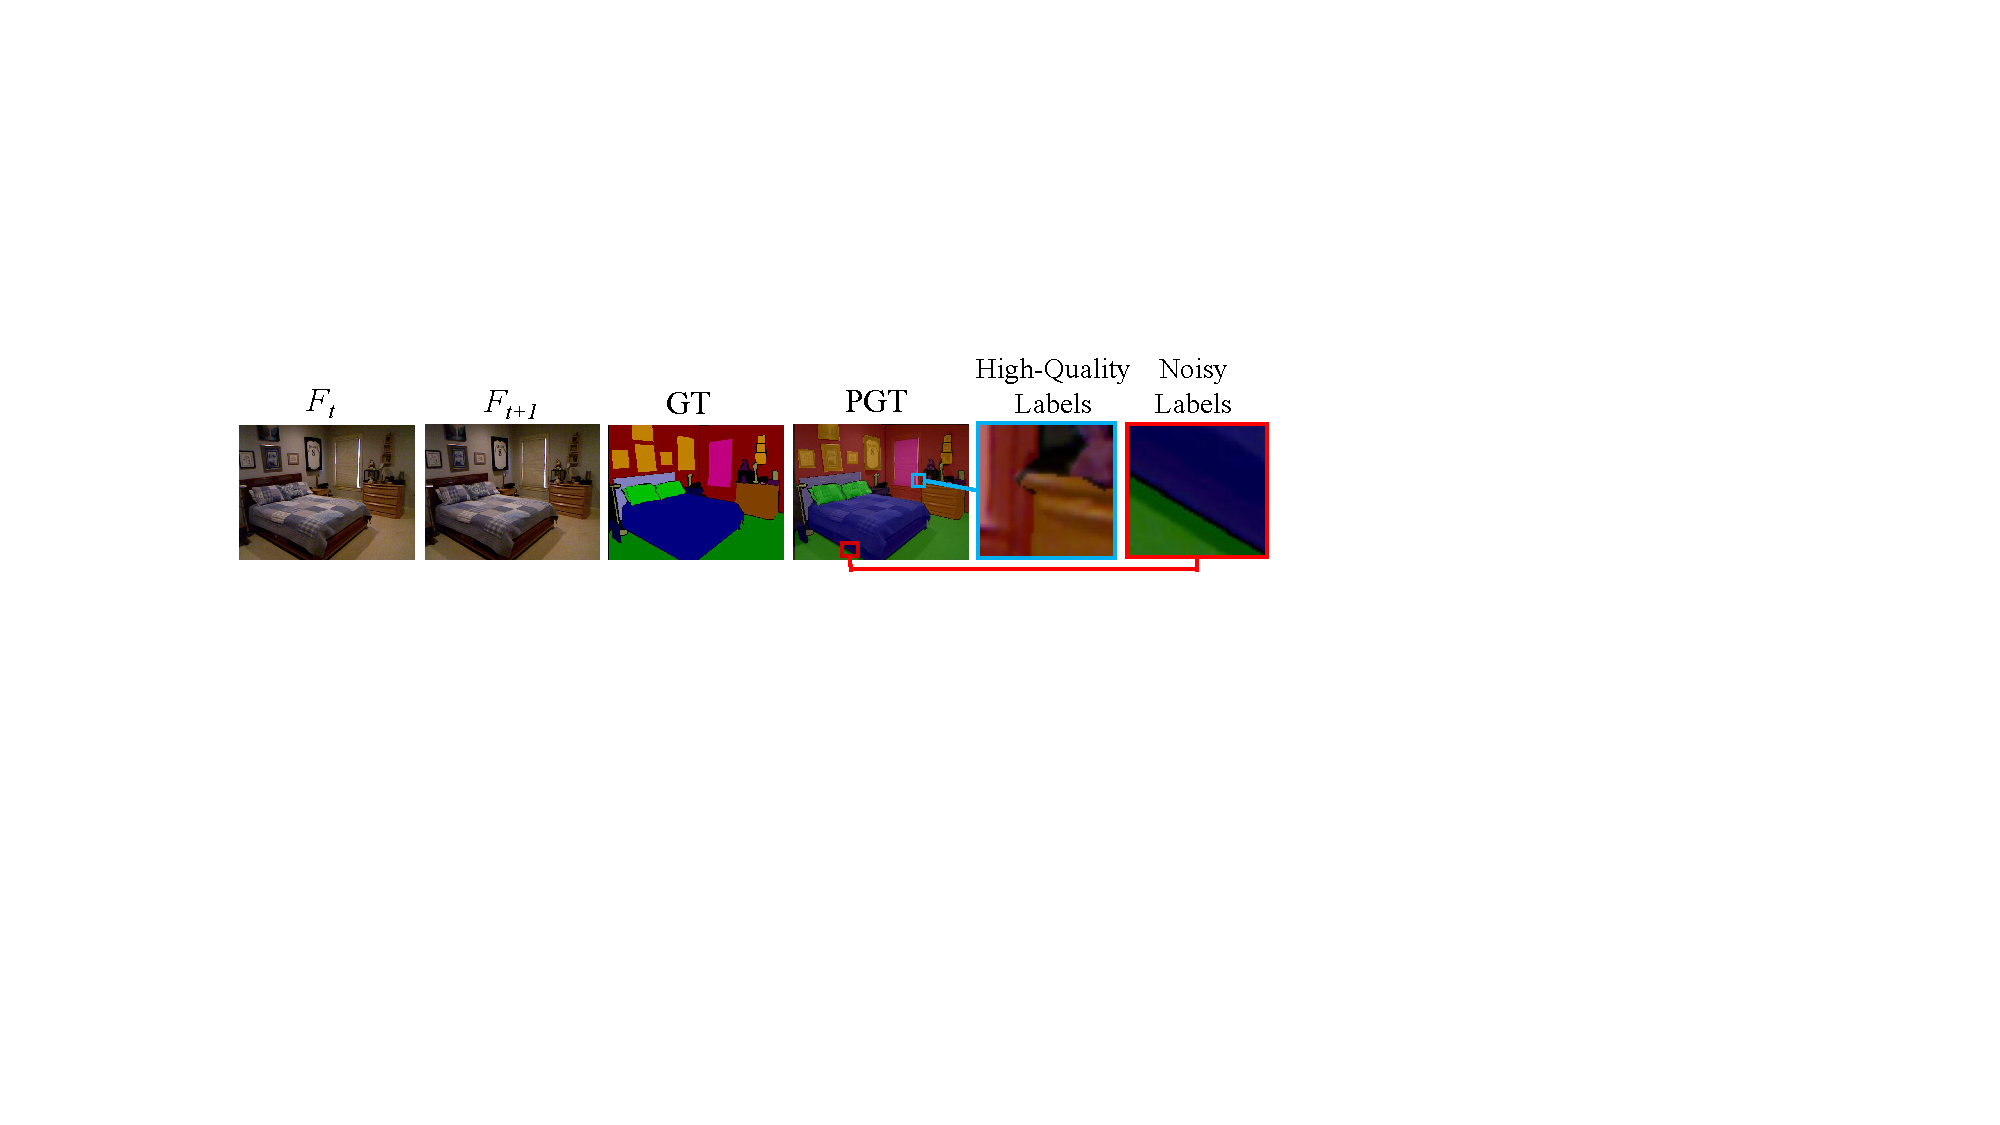
\includegraphics[width=\columnwidth]{figure/PGT.pdf}
	%	\vspace*{-0.6cm} 
	\caption{Propagated pseudo ground truth from a reference frame $F_t$ to $F_{t+1}$. Most of the pseudo labels are reliable, while there are some noisy around object boundaries.}
	\label{fig:PGT}
	%	\vspace*{-0.35cm} 
\end{figure}

%\noindent\textbf{Training Segmentation Network using Temporal Consistency.}
\subsection{Training Segmentation Network using Temporal Consistency}
%
As Fig.~\ref{fig:Pipeline} shows, we train a semantic segmentation network using two adjacent frames in a video instead of using a single labeled frame to exploit the interconnection of them.  
% 
First, two adjacent frames $F_{t-1}$ and $F_t$ are passed through a basic segmentation network to predict semantic labels $S_{t-1}$ and $S_{t}$.
%
The basic segmentation network could be any existing semantic segmentation model. 
%
In this work, we use RDFNet\cite{Park2017}, which is a high-precision network for semantic segmentation of a RGBD image.

\begin{figure}[t]
	\centering
	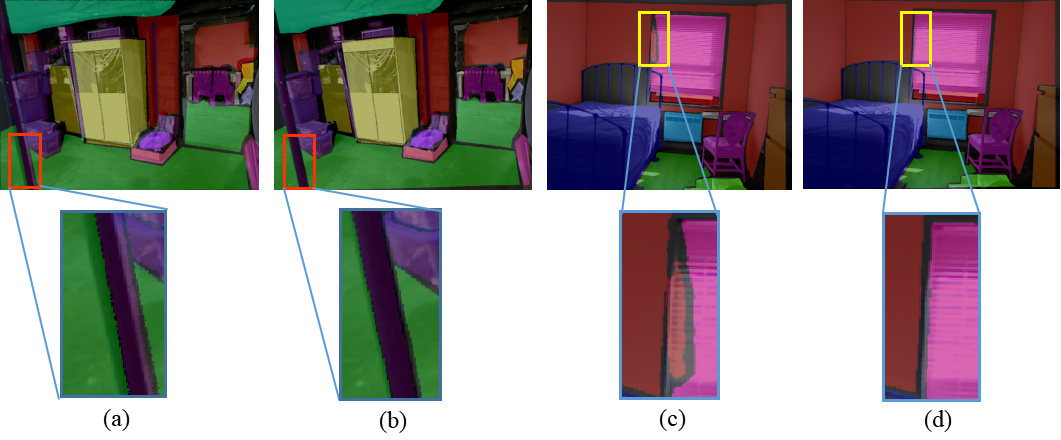
\includegraphics[width=\columnwidth]{figure/PGT_compared.png}
	%	\vspace*{-0.6cm} 
	\caption{Comparison of different methods of annotation propagetion. (a) PGT generated by rigid body transformation. The camera external parameters are evaluated by Bundler and the depth is filled using NYU-v2 official code. (b)(d) PGT of our method. (c) PGT generated by optical flow using PWC-Net\cite{Sun2018}. The blue boxes are zoomed-in figures showing the details.}
	\label{fig:PGT_Com}
	%	\vspace*{-0.35cm} 
	
\end{figure}
Second, the predicted semantic score map $S_{t-1}$ for frame $F_{t-1}$ is warped to $\hat{S}_{t}$ according to the optical flow $O_{t-1,t}$ between $F_t$ and $F_{t-1}$, which is estimated using an efficient and accurate model PWC-Net~\cite{Sun2018} from two frames. 
We implement a bilinear interpolation for $40$ dimensional score vector of each pixel in $S_{t-1}$, where 40 is the total number of object classes in the dataset. 
\begin{equation}
\centering
\hat{S}_{t}=Warp(S_{t-1},O_{t-1,t}).
\end{equation}
%
An argmax layer is then added on the warped score map ${\hat{S}_{t}}$ to generate the warped semantic prediction $W_{t}$.
\begin{comment}
\begin{equation}
\centering
W_{t}=\arg \max \hat{S}_{t-1}.
\end{equation}
\end{comment}


Finally, the warped prediction $W_{t}$ acts as a self-supervised item to constrain the consistency of prediction results between neighboring video frames.
%
Meanwhile, the PGT of current frame $F_t$ acts as another supervisory item to guarantee that the prediction results are as accurate as possible.
Combining these two items, our loss function is defined as
\begin{equation}
\centering
\begin{aligned}
L_{seg}= \lambda L_{Consistency} +(1-\lambda)L_{PGT},
\end{aligned}
\end{equation}
%
where, ${L_{PGT}}$ and ${L_{Consistency}}$ are cross-entropy loss, defined as
\begin{equation}
{
\vspace*{-0.6cm} 
\centering     
\begin{aligned} 
L_{Consistency} &= -\sum_{i=0} l(\mathbf{w}_i,\mathbf{y}_i),\\
L_{PGT} = -&\sum_{i=0} l(\mathbf{p}_i,\mathbf{y}_i), \\
l(\mathbf{p}_i,\mathbf{y}_i) = -&\sum_{k=0}^c \,\mathbf{p}_{ik}\log{\mathbf{y}_{ik}}\;,\; \mathbf{y}_{i} = f(x_{i}),\\
\end{aligned}
}
\end{equation}
%
where ${x_i}$ and ${\mathbf{y}_i}$ are a pixel of an input frame and the corresponding predicted output of the semantic segmentation model respectively. 
%
$\mathbf{y}_i$ is a $c$ dimensional probability vector for each pixel.
${c}=40$ is number of categories.
%
${\mathbf{p}_i}$ and ${\mathbf{w}_i}$ are one-hot vectors for each pixel of the pseudo ground truth or ground truth label, and warped prediction $W_{t}$ from previous frame, respectively. 
%
${l(\cdot)}$ is the softmax loss of one pixel, and ${f(\cdot)}$ is our basic segmentation network. 
%
By these two losses, we can constrain the accuracy and temporal consistency of the network prediction simultaneously.
